\chapter{Development}\label{Development}
\section{Component List}
\subsection{Introduction}
To create the basis for development of this project two microphones and a structure to keep a constant distance between them were necessary.  
\subsection{Distancing}
To maintain a constant distance it was decided to attempt modeling a rod with two microphone holders at it's ends. The distance chosen between the microphones was agreed on by referring to a research article in this area: 15.2 centimeters. 
\paragraph{}
Other parameters were found by following the measurements found in the datasheet[ref].
\begin{figure}[ref] {r}
  \caption{A picture of a gull.}
  \centering
    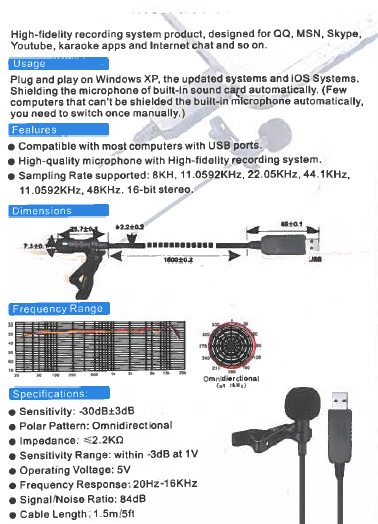
\includegraphics[width=0.5\textwidth]{Illustrations/MicData}
\end{figure}

\todo[inline,color=green]{\url{https://www.researchgate.net/publication/228749231_Analysis_of_the_Facial_Anthropometric_Data_of_Korean_Pilots_for_Oxygen_Mask_Design}}
\subsection{Microphones characteristics}
\subsection{Measurements scenarios}
\subsection{Setup}
\section{Analog to digital conversion}



